% Editable native annotations around unchanged verified IDE photographs.
\par
\begin{figure}[htbp]
\centering
\sbox0{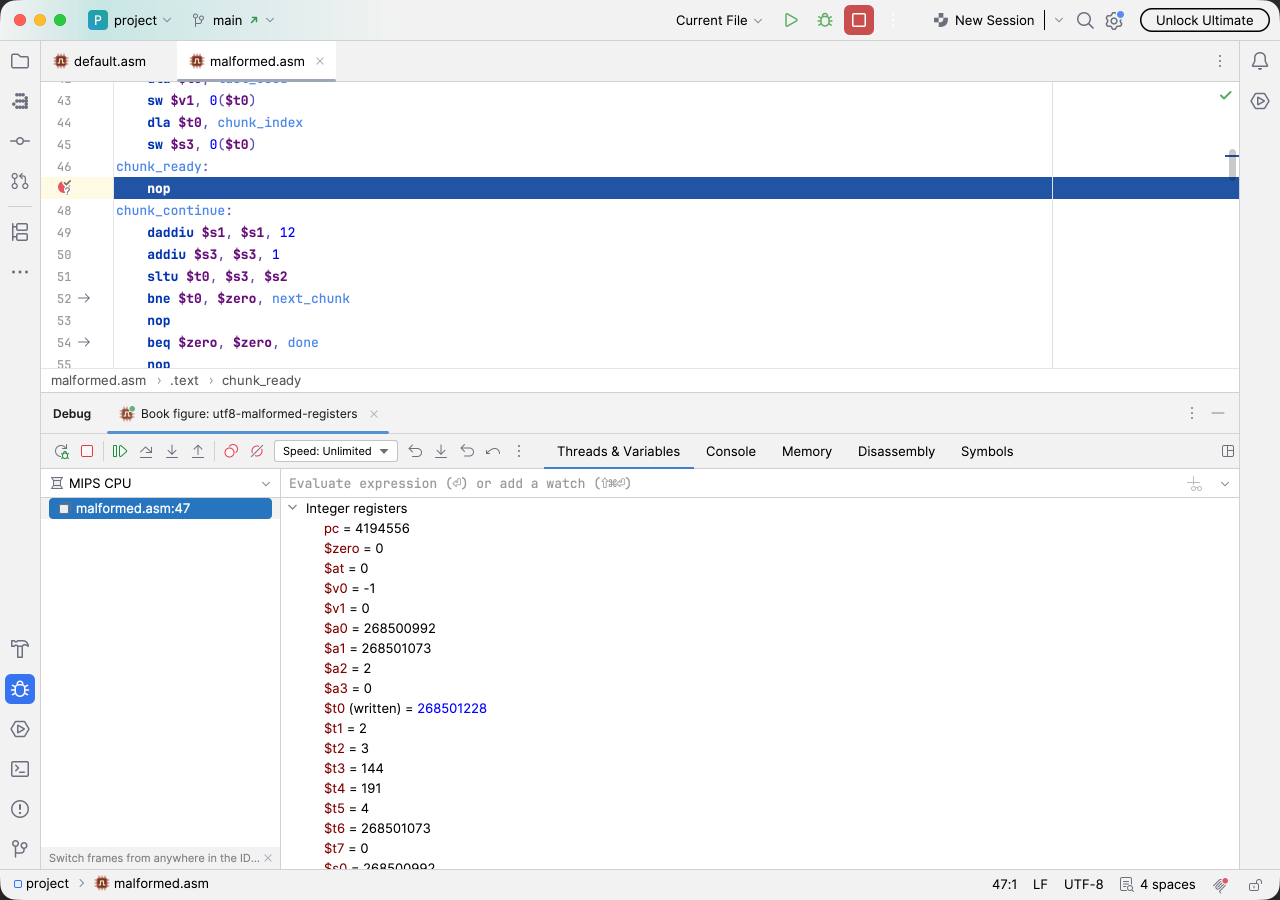
\includegraphics[artifact]{packages/015-utf8-scanner/captures/f03-malformed/registers.png}}
\sbox2{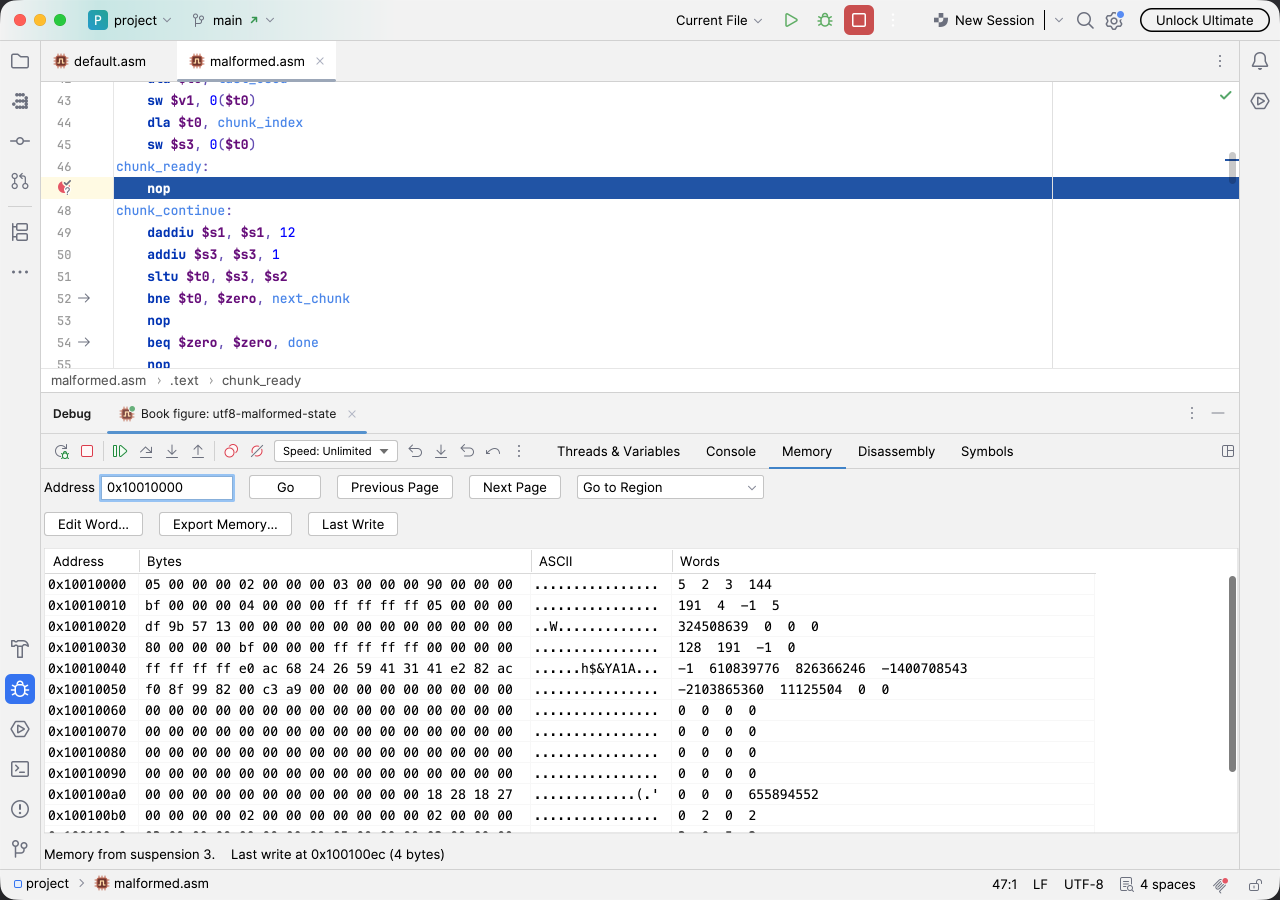
\includegraphics[artifact]{packages/015-utf8-scanner/captures/f03-malformed/state.png}}
\sbox4{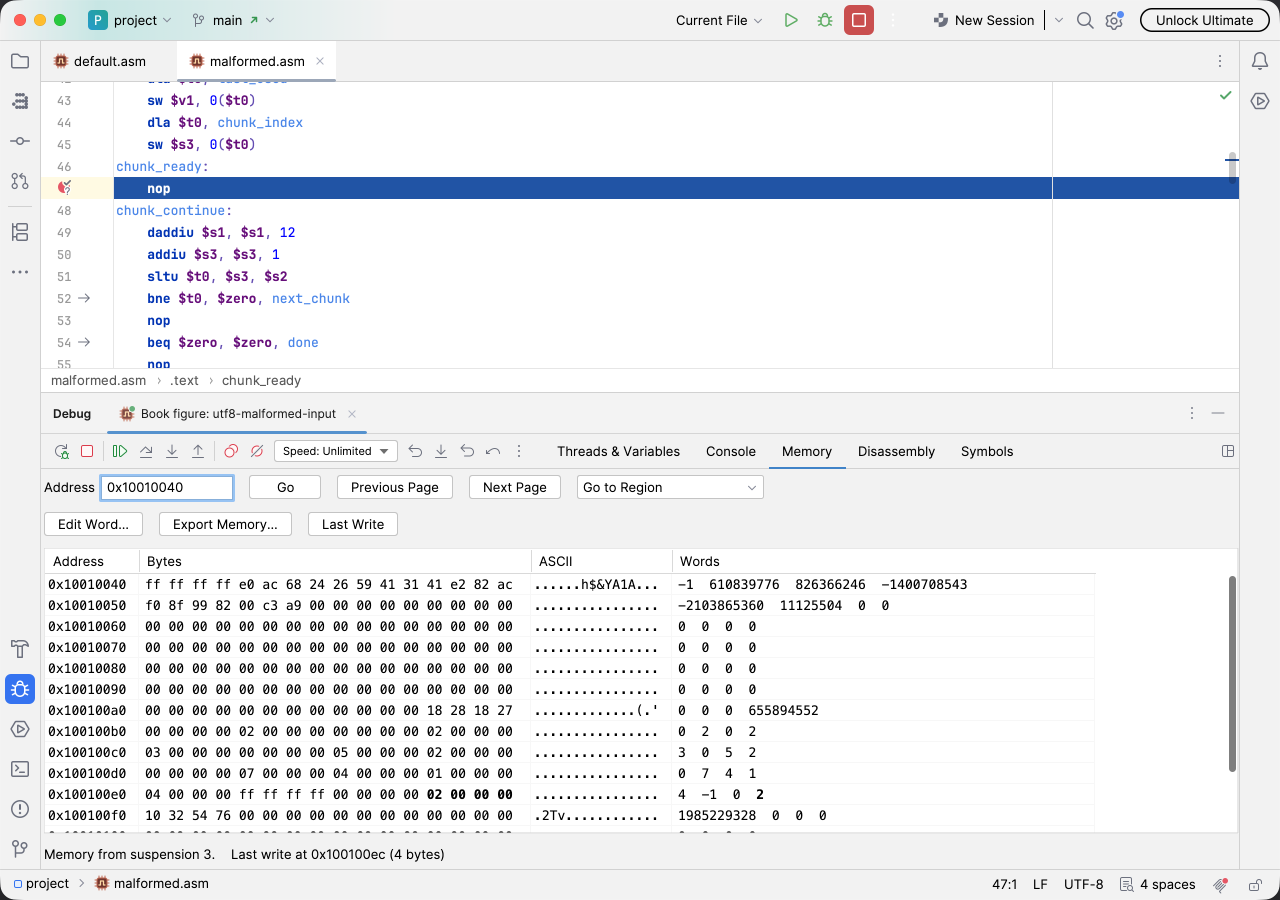
\includegraphics[artifact]{packages/015-utf8-scanner/captures/f03-malformed/input.png}}
\edef\MARSutfmalformedsourceLeft{\the\dimexpr0.036718750\wd0\relax}
\edef\MARSutfmalformedsourceBottom{\the\dimexpr0.774444444\ht0\relax}
\edef\MARSutfmalformedsourceRight{\the\dimexpr0.713281250\wd0\relax}
\edef\MARSutfmalformedsourceTop{\the\dimexpr0.147777778\ht0\relax}
\edef\MARSutfmalformedregistersLeft{\the\dimexpr0.246093750\wd0\relax}
\edef\MARSutfmalformedregistersBottom{\the\dimexpr0.312222222\ht0\relax}
\edef\MARSutfmalformedregistersRight{\the\dimexpr0.553906250\wd0\relax}
\edef\MARSutfmalformedregistersTop{\the\dimexpr0.640000000\ht0\relax}
\edef\MARSutfmalformedstateLeft{\the\dimexpr0.034375000\wd2\relax}
\edef\MARSutfmalformedstateBottom{\the\dimexpr0.311111111\ht2\relax}
\edef\MARSutfmalformedstateRight{\the\dimexpr0.584375000\wd2\relax}
\edef\MARSutfmalformedstateTop{\the\dimexpr0.608888889\ht2\relax}
\edef\MARSutfmalformedinputLeft{\the\dimexpr0.034375000\wd4\relax}
\edef\MARSutfmalformedinputBottom{\the\dimexpr0.311111111\ht4\relax}
\edef\MARSutfmalformedinputRight{\the\dimexpr0.584375000\wd4\relax}
\edef\MARSutfmalformedinputTop{\the\dimexpr0.608888889\ht4\relax}
\begin{tikzpicture}[alt={Four annotated details after chunk index two with only input byte five changed from 9f to 8f. Native return status minus one and used zero accompany state total five, count two, need three, permitted range 144 through 191, start four, malformed status minus one and error five. The detecting byte 8f is not accepted and its suffix is not read.}]
\node[anchor=north west,inner sep=0,font=\small\bfseries] (source-title) at (6mm,0) {Next instruction after publication};
\node[anchor=north west,inner sep=0] (source) at ([yshift=-1mm]source-title.south west) {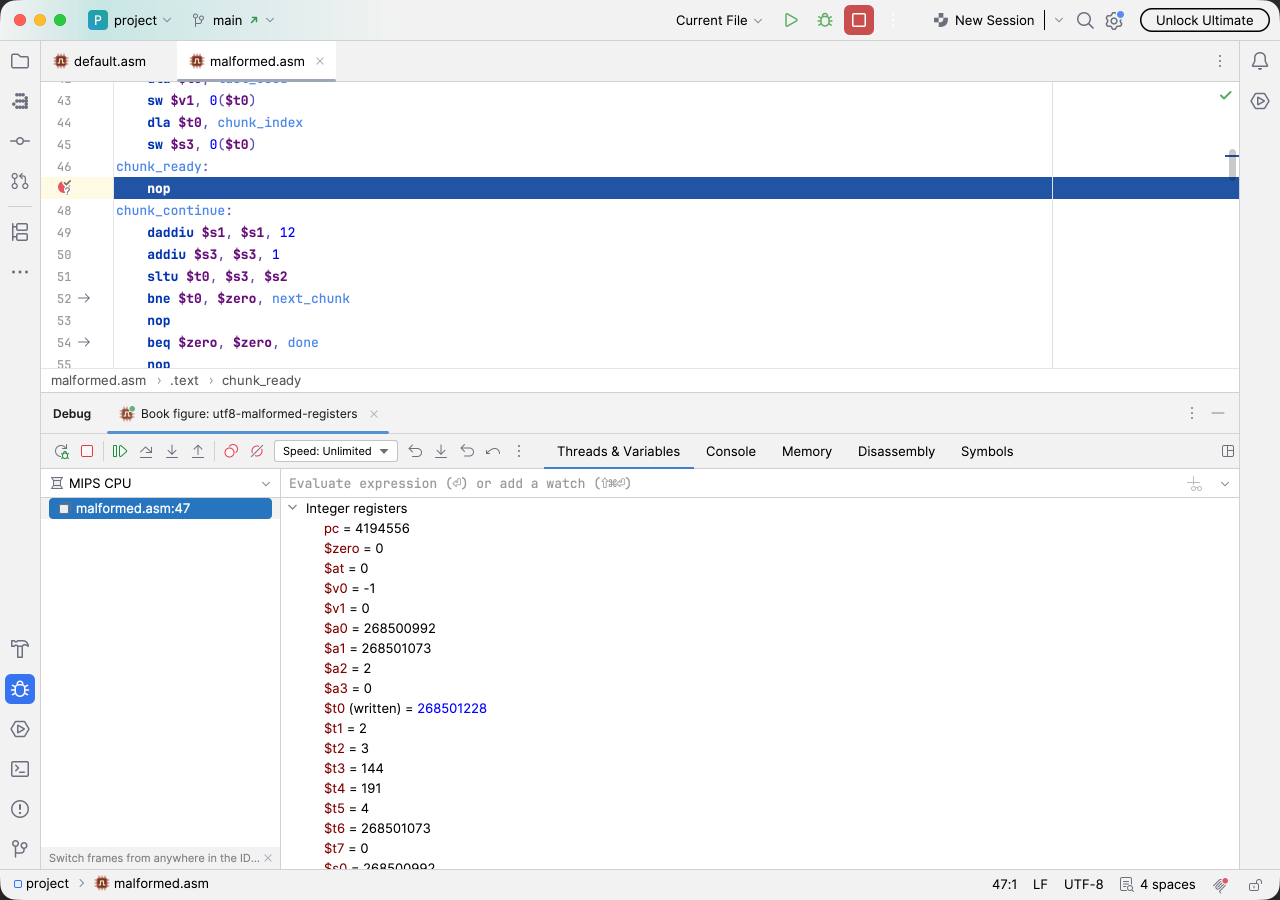
\includegraphics[width=0.54\linewidth,artifact,trim={\MARSutfmalformedsourceLeft{} \MARSutfmalformedsourceBottom{} \MARSutfmalformedsourceRight{} \MARSutfmalformedsourceTop{}},clip]{packages/015-utf8-scanner/captures/f03-malformed/registers.png}};
\begin{scope}[shift={(source.south west)},x={($(source.south east)-(source.south west)$)},y={($(source.north west)-(source.south west)$)}]
\draw[black,line width=0.7pt] (0.215625000,0.057142857) rectangle (0.384375000,0.371428571);
\node[draw=black,fill=white,circle,inner sep=1.5pt,font=\footnotesize] at ($(0.215625000,0.371428571)+(-3mm,0)$) {1};
\end{scope}
\node[anchor=north west,inner sep=0,font=\small\bfseries] (registers-title) at (0.58\linewidth,0 |- source-title.north) {Signed return values};
\node[anchor=north west,inner sep=0] (registers) at ([yshift=-1mm]registers-title.south west) {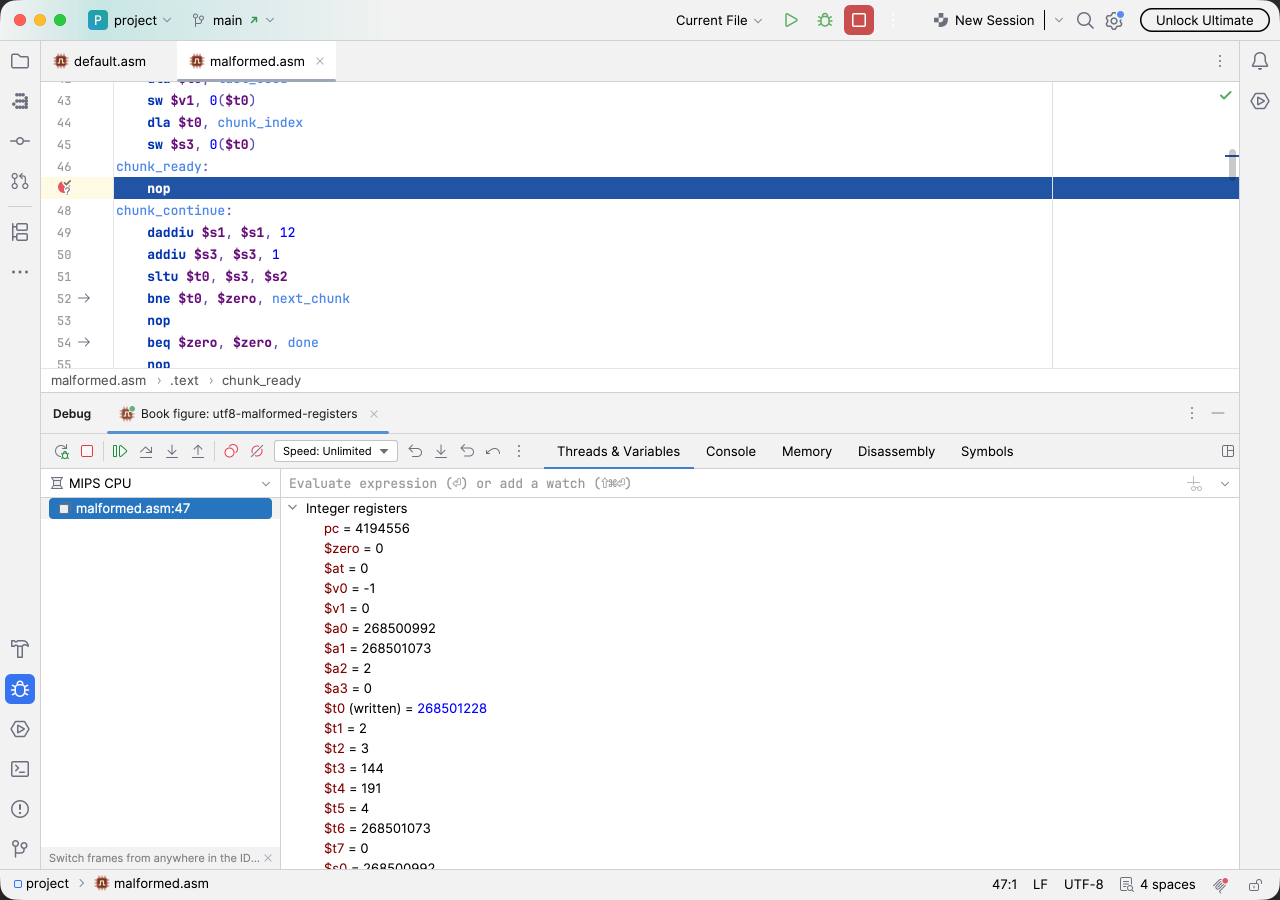
\includegraphics[width=0.42\linewidth,artifact,trim={\MARSutfmalformedregistersLeft{} \MARSutfmalformedregistersBottom{} \MARSutfmalformedregistersRight{} \MARSutfmalformedregistersTop{}},clip]{packages/015-utf8-scanner/captures/f03-malformed/registers.png}};
\begin{scope}[shift={(registers.south west)},x={($(registers.south east)-(registers.south west)$)},y={($(registers.north west)-(registers.south west)$)}]
\draw[black,line width=0.7pt] (0.023437500,0.023255814) rectangle (0.242187500,0.953488372);
\node[draw=black,fill=white,circle,inner sep=1.5pt,font=\footnotesize] at ($(0.023437500,0.953488372)+(-3mm,0)$) {2};
\end{scope}
\node[anchor=north west,inner sep=0,font=\small\bfseries] (state-title) at ([yshift=-3mm]source.south west) {Stream state: eight little-endian words};
\node[anchor=north west,inner sep=0] (state) at ([yshift=-1mm]state-title.south west) {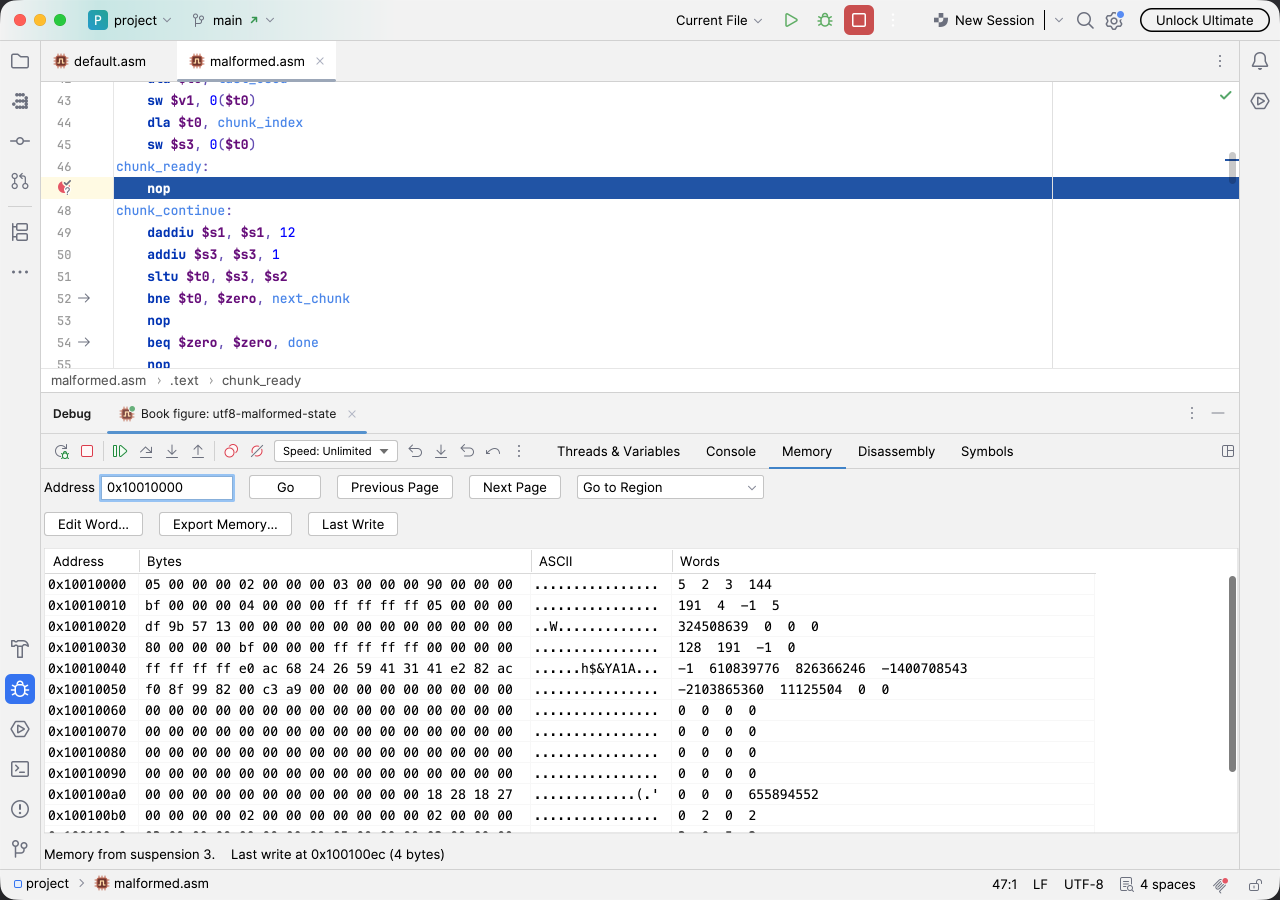
\includegraphics[width=0.84\linewidth,artifact,trim={\MARSutfmalformedstateLeft{} \MARSutfmalformedstateBottom{} \MARSutfmalformedstateRight{} \MARSutfmalformedstateTop{}},clip]{packages/015-utf8-scanner/captures/f03-malformed/state.png}};
\begin{scope}[shift={(state.south west)},x={($(state.south east)-(state.south west)$)},y={($(state.north west)-(state.south west)$)}]
\draw[black,line width=0.7pt] (0.194672131,0.055555556) rectangle (0.997950820,0.638888889);
\node[draw=black,fill=white,circle,inner sep=1.5pt,font=\footnotesize] at ($(0,0.638888889)+(-3mm,0)$) {3};
\end{scope}
\node[anchor=north west,inner sep=0,font=\small\bfseries] (input-title) at ([yshift=-3mm]state.south west) {Mapped input and neighboring words};
\node[anchor=north west,inner sep=0] (input) at ([yshift=-1mm]input-title.south west) {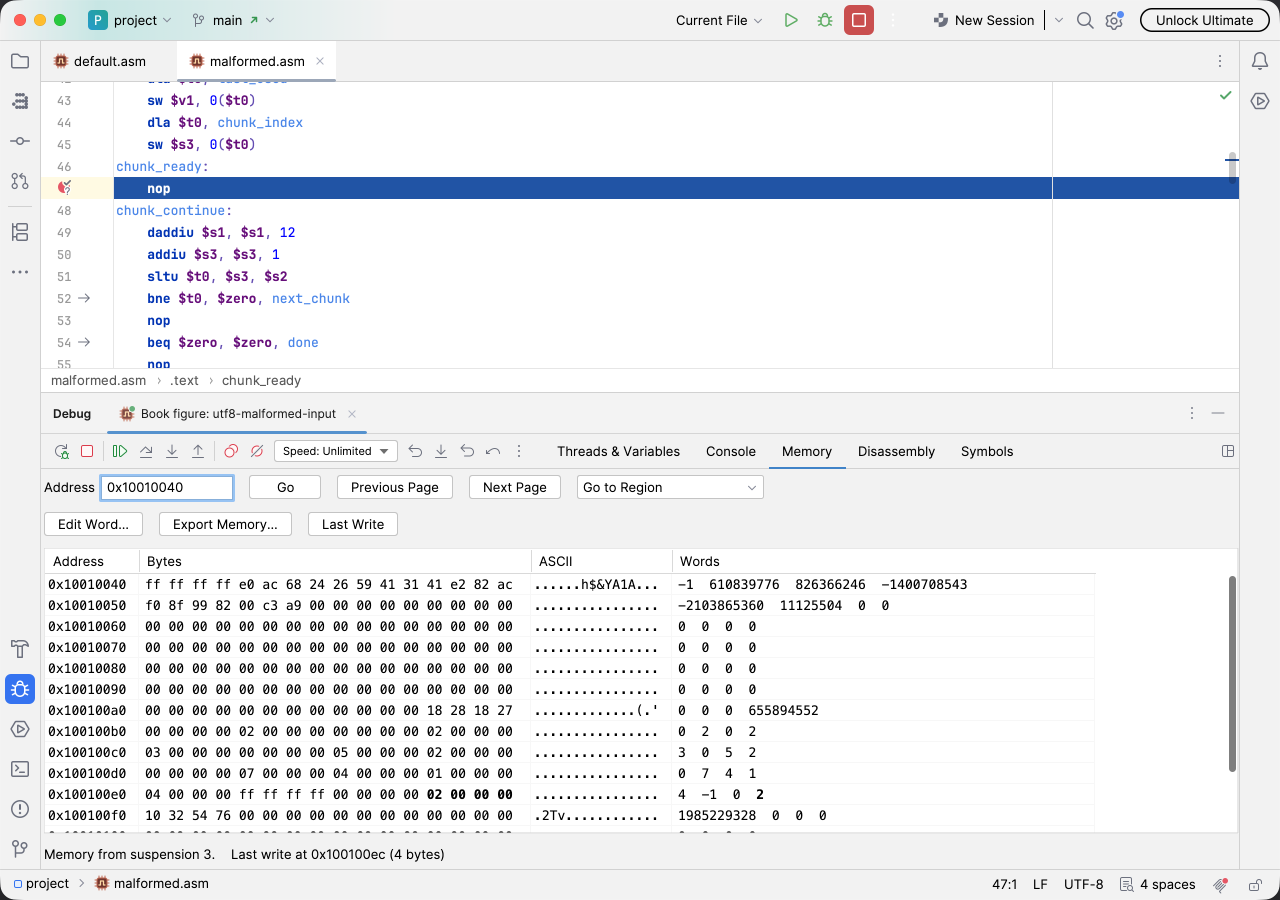
\includegraphics[width=0.84\linewidth,artifact,trim={\MARSutfmalformedinputLeft{} \MARSutfmalformedinputBottom{} \MARSutfmalformedinputRight{} \MARSutfmalformedinputTop{}},clip]{packages/015-utf8-scanner/captures/f03-malformed/input.png}};
\begin{scope}[shift={(input.south west)},x={($(input.south east)-(input.south west)$)},y={($(input.north west)-(input.south west)$)}]
\draw[black,line width=0.7pt] (0.194672131,0.055555556) rectangle (0.997950820,0.638888889);
\node[draw=black,fill=white,circle,inner sep=1.5pt,font=\footnotesize] at ($(0,0.638888889)+(-3mm,0)$) {4};
\end{scope}
\end{tikzpicture}
\par\smallskip
\begin{minipage}{\linewidth}
\small
\begin{enumerate}
\setlength{\itemsep}{2pt}
\setlength{\parsep}{0pt}
\item This fixture changes only input byte 5 from \texttt{9f} to \texttt{8f}. The first two calls reach the same pending state as the valid stream. The stop follows chunk index 2, the third call, at the same \texttt{chunk\_ready} publication boundary.
\item The native signed-decimal return values are \texttt{\$v0 = -1} and \texttt{\$v1 = 0}: malformed input, with no bytes accepted from this call. The detecting byte is inspected to decide the result but is excluded from the accepted count. The remaining byte of the offered chunk is not read.
\item The state is $[5,2,3,144,191,4,-1,5]$. Total remains 5 and count remains 2. Start 4 still identifies the accepted \texttt{f0} lead; error 5 identifies the byte that makes completion impossible. Both are absolute stream offsets, not MIPS memory addresses. The pending count and bounds retain the context of that failure.
\item The second displayed row begins at \texttt{0x10010050}: its first bytes are \texttt{f0 8f 99 82}. The changed \texttt{8f} at address \texttt{0x10010051} has continuation-byte form, yet lies below the required minimum \texttt{90} after \texttt{f0}. Such a prefix cannot form a shortest four-byte encoding. The scanner reports that earliest impossible byte; the trace confirms no read of its suffix.
\end{enumerate}
\end{minipage}
\caption{An impossible continuation is detected at offset five; its sequence began at four.}
\label{capture:015-utf8-scanner-f03-malformed}
\label{utf8-f03-malformed}
\end{figure}
\par
